% coding:utf-8

%----------------------------------------
%FOSADSVB, a LaTeX-Code for a summary of digital signal processing
%Copyright (C) 2015, Mario Felder & Michi Fallegger

%This program is free software; you can redistribute it and/or
%modify it under the terms of the GNU General Public License
%as published by the Free Software Foundation; either version 2
%of the License, or (at your option) any later version.

%This program is distributed in the hope that it will be useful,
%but WITHOUT ANY WARRANTY; without even the implied warranty of
%MERCHANTABILITY or FITNESS FOR A PARTICULAR PURPOSE.  See the
%GNU General Public License for more details.
%----------------------------------------

\chapter{Digitale Signale im Zeitbereich}
\section{Signal Analyse}
\subsection{Sampling}
Die Sample-Frequenz $f_S$ ist durch die Sample-Periode
$T_S$ gegeben:
\[ f_S = \frac{1}{T_S} \]
Aus dem Signal $x(t)$ wird durch die Abtastung:
\[ x(n\cdot T_S) = x[n]\]
Das Signal $x[n]$ ist kausal wenn:
\[ x[n] = 0 \qquad \textrm{für alle } n < 0 \]

%===============================================================================
\subsection{Standard digital Signale}
Einheitsimpuls oder Diracimpuls:
\[
	\delta = \left\lbrace \begin{matrix}
		0 & : & n \neq 0 \\
		1 & : & n = 0
	\end{matrix} \right.
\]
Einheitsschirtt:
\[
	\delta = \left\lbrace \begin{matrix}
		0 & : & n < 0 \\
		1 & : & n \geq 0
	\end{matrix} \right.
\]
Ein periodisches Signal ist beschrieben durch:
\[ x[n] = x[n + T_0/T_S] \qquad \textrm{mit } T_0/T_S = k \]
Ein periodisches Signal muss eine Periodendauer $T_0$ haben,
welche ein ganzzahliges Vielfaches der Sample-Periode $T_S$ ist. 

\begin{center}
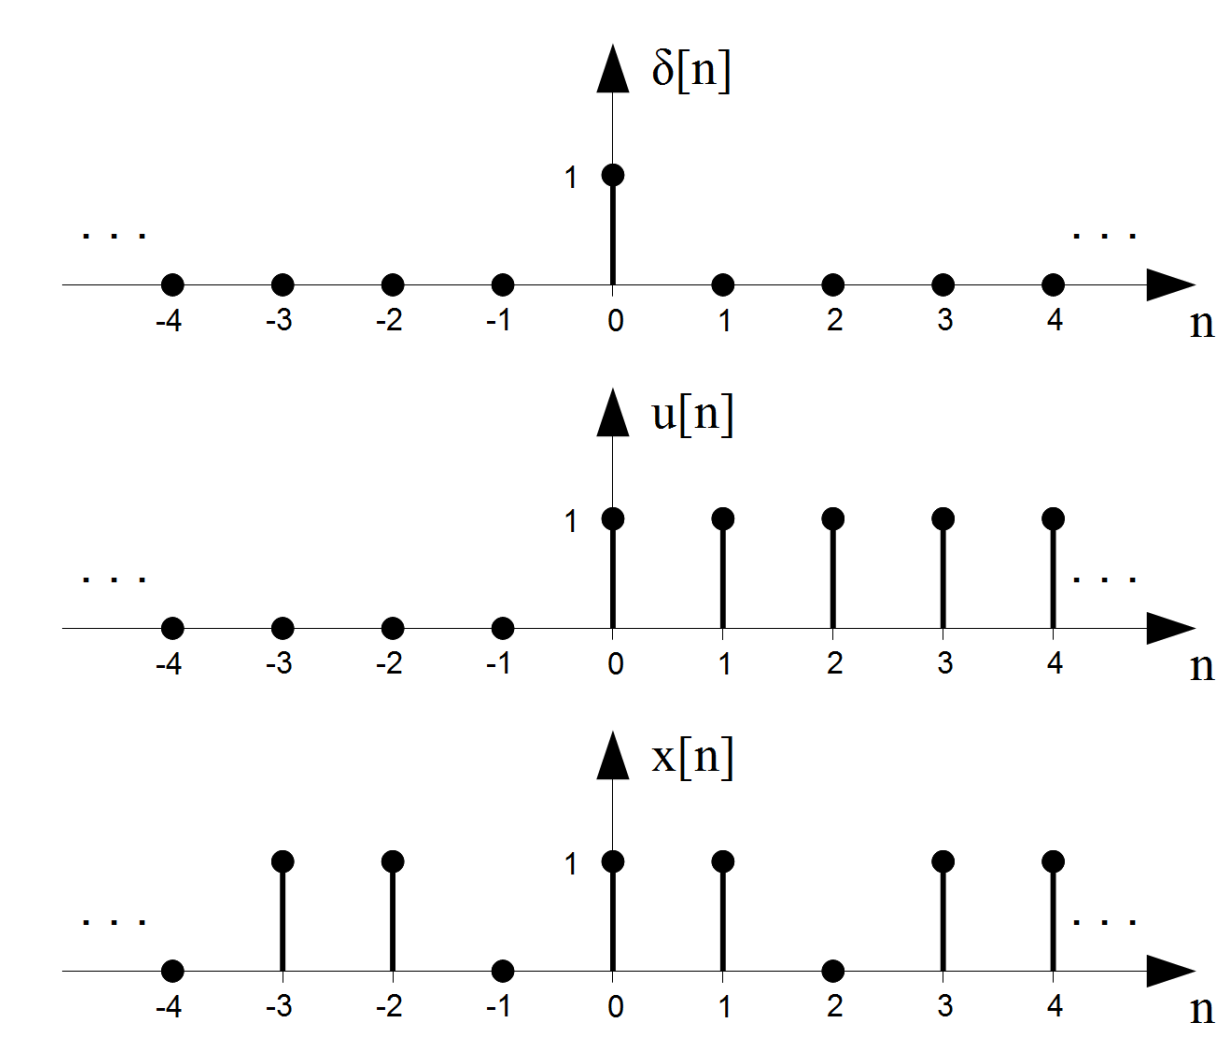
\includegraphics[scale=.7]{./images/basic_signals}
\end{center}

Komplexe harmonische Sequenz:
\[ x[n] = \hat{X} \cdot \e^{\im 2 \pi f_0 n T_S} \]
Real- und Imaginäranteil der komplexen Harmonischen:
\[ Re\{\} = \hat{X} \cdot \cos 2 \pi f_0 n T_S \]
\[ Im\{\} = \hat{X} \cdot \sin 2 \pi f_0 n T_S \]

%===============================================================================
\subsection{Statistische Signalparameter}
Observations Intervall $T$:
\[ T = N \cdot T_S \]
Der Mittelwert (\textbf{mean value}) $\mu_x$ repräsentiert
den DC-Anteil des Signals x[n]:
\[ \mu_x = \frac{1}{N} \sum_{i=0}^{N-1}x[i] \]
Der quadratische Mittelwert (\textbf{quadratic mean value}) ${\rho_x}^2$
korrespondiert zur durchschnittlichen Leistung des Signal $x[n]$
mit DC-Anteil:
\[ {\rho_x}^2 = \frac{1}{N} \sum_{i=0}^{N-1} x[i]^2 \]
Die \textbf{Varianz} ${\sigma_x}^2$ repräsentiert die durchschnittliche
AC-Leistung des Signals $x[n]$:
\[ {\sigma_x}^2 = \frac{1}{N} \sum_{i=0}^{N-1}(x[i] - \mu_x)^2 \]

%===============================================================================
\subsection{Messverhältnisse und dB}
Leistungsverhältnis (\textbf{power ratio}):
\[ A_{dB} = 10 \cdot \log_{10} \left( \frac{P_1}{P_2} \right) \]
Signal-to-noise ratio (\textbf{SNR}):
\[ SNR_{dB} = 10 \cdot \log_{10} \left( \frac{P_{signal}}{P_{noise}} \right) \]

\begin{table}[ht]
  \centering
  \begin{tabular}{ccc} \toprule
  Linear	& \multicolumn{2}{c}{Power ratio [dB]} \\ 
  $a/b$		& Power		& Voltage	\\ \midrule
  $1/1000$	& -30		& -60		\\
  $1/100$	& -20		& -40		\\
  $1/10$	& -10		& -20		\\
  $1/2$		& $\approx -3$& $\approx -6$\\
  $1$		& 0			& 0			\\
  $2/1$		& $\approx -3$& $\approx 6$\\
  $10/1$	& 10		& 20		\\
  $100/1$	& 20		& 40		\\  \bottomrule
  \end{tabular}
\end{table}

%===============================================================================
\section{Signal Operationen}
\subsection{Korrelation}
Die statische Korrelation (\textbf{static correlation}) drückt die Ähnlichkeit
zweier Signale x[n] und y[n] der selben Länge $N$ aus:
\[ R = \frac{1}{N} \sum_{i=0}^{N-1} x[i]y[i] \]
Je ähnlicher sich die Signale sind, desto grösser der Wert $R$.\\\\
Die lineare Korrelationsfunktion (\textbf{linear correlation fucntion}):
\[ r_{xy}[n] = \sum_{i=-\infty}^{\infty} x[i]y[i+n] \]
Die Korrelation ist nicht kommutativ, $r_{xy}[n] \neq r_{yx}[n]$.\\\\
Resultierende Länge von $r_{xy}$:
\[ N_{xy} = N_x + N_y - 1 \]
~\\
Mathlabbefehl für Kreuz- und Autokorrelation: \verb|xcorr|

\subsection{Faltung}
Die Faltung (\textbf{convolution}) ist definiert als:
\[ z[n] = \sum_{i=-\infty}^{\infty} x[i]y[-i+n] \]
Die Faltung ist kommutativ:
\[ z[n] = x[n] * y[n] = y[n] * x[n] \]
Resultierende Länge für $z[n]$:
\[ N_z = N_x + N_y -1 \]
Bei der zyklischen Faltung (\textbf{circular convolution}) müssen die beiden
Signale die selbe Länge $N$ haben, oder mit Zero-Padding auf die selbe Länge
gebracht werden:
\[ z[n] = x[n] \circledast_N y[n] = y[n] \circledast_N x[n] \]
Lösung durch Matrix:
\[
	\begin{bmatrix}
		y[N]	& y[N-1]	& \ldots & y[0] \\
		y[0]	& y[N]		& \ddots & y[1] \\
		\ddots	& \ddots	& \ddots & \ddots \\
		y[N-1]	& y[N-2]	& \ldots & y[N]
	\end{bmatrix} \cdot \begin{bmatrix}
		x[0] \\ x[1] \\ \vdots \\ x[N]
	\end{bmatrix} = \begin{bmatrix}
		z[0] \\ z[1] \\ \vdots \\ z[N]
	\end{bmatrix}
\]
~\\\\
Mathlabbefehl für Faltung: \verb|conv|\\
Mathalbbefehl für zyklische Faltung: \verb|convmtx|